\documentclass[12pt]{elsarticle}
\usepackage{graphicx}
\usepackage{amssymb}
\usepackage{lineno}
\usepackage{amsmath} 
\usepackage{graphicx}
\usepackage{amsmath,amssymb}
\DeclareMathOperator{\E}{\mathbb{E}}

%opening
\journal{STAT 520A}

\begin{document}
	
\begin{frontmatter}
\title{A Benchmarking comparison of MCMC and SMC Samplers}
\author{Jason Hartford - 81307143 \\ Dustin Johnson - 11338118}

\begin{abstract}
In this paper, we compare and contrast two major sampling methods for posterior inference, namely Markov Chain Monte Carlo (MCMC) and Sequential Monte Carlo (SMC) samplers based on their performance and efficiency under a series of artificial density functions. Increasing distributional complexity of Bayesian modeling has demanded improvements in the efficiency and performance of sampling methods.  The purpose of the paper is to determine preference of one method over the other through experiments on artificial density functions of varying dimensions. The algorithms are implemented and benchmarked in the language Julia, a rather new and emerging language with demonstrated potential for statistical computing.
\end{abstract}

\begin{keyword}
MCMC \sep SMC Samplers \sep Bayesian Analysis \sep Julia
\end{keyword}

\end{frontmatter}



\section*{Introduction}
Markov Chain Monte Carlo (MCMC) has become a favoured tool for Statisticians when sampling from complex distributions by constructing an ergodic Markov chain with an invariant distribution through Metropolis-Hasting (MH) steps. It is for this reason that MCMC has become the standard sampling technique that has enabled Bayesian statistics to evolve and be applied to increasingly complex and higher dimensional problems. However, MCMC has been shown to get stuck in local modes and difficulty arises when assessing whether the Markov chain has truly reached its stationary distribution. In addition, the full joint distribution must be evaluated each time a new variable is added, which is infeasible under a sequential context. \\

Escalating interest in Bayesian modeling has increased the complexity of the posterior distributions, where multiple modes in high dimensional space are common. This complexity has placed higher demands for improvements in sampling methods in terms of performance and computational efficiency. Sequential Monte Carlo (SMC) samplers offer an alternative to MCMC by offering the ability to sample from a posterior distribution through a novel online algorithm, as opposed to sampling from the entire joint distribution each time new observations enters the model.  Additionally, SMC sSaplers have been shown to cover multiple modes with improved efficiency due to the reweighing of particles after each iteration of the algorithm. \\

In the sections to follow, we will provide a brief outline of MCMC and SMC samplers, then compare and contrast their performance under a series of experiments with artificial density functions of varying dimensions.

\section*{Markov Chain Monte Carlo (MCMC)}
MCMC accomplishes the task of approximating the area of an unknown distribution by moving through the space of the joint distribution by a series of carefully taken steps. Each "chain" of steps is an MCMC sampler if they are ergodic Markov chains (irreducible and aperiodic) that have the target distribution as the invariant distribution.  We will focus on the most popular MCMC method, called the Metropolis-Hastings (MH) algorithm. Most other MCMC methods can be viewed as special cases of this algorithm (Andrieu, et al. 2003). \\

Let $x'$ be the proposal candidate for the next step of the Markov chain, which is drawn from the proposal distribution denoted $q(x'|x)$, where $x$ is our current point. This proposal is then accepted as the next step in the Markov chain according to the probability $\alpha(x,x')$, where 

\[
\alpha(x,x') = \min{\left[1, \frac{\pi(x') q(x|x')}{\pi(x)q(x'|x)}\right]} \quad (1)
\].

If the proposal candidate is rejected, then the next sampled value is taken to be the current value. We iterate this process until some form of convergence is reached (see section Convergence Benchmarks). Typically, a Markov chain takes a number of steps from the initial point before reasonably traversing the area and converging to the invariant distribution, so a sequence of the initial steps is discarded called the ``burn-in" period. It is important to note that the target density appears as a ratio in the probability $ \alpha(x,x')$ and therefore the algorithm can be implemented without the normalizing constant $Z = \int \mathcal{L}(x|\theta)\pi(\theta)$ inherent in a Bayesian framework.

\section*{Sequential Monte Carlo (SMC) Samplers}
The search for improved sampler performance and alternative methods to circumvent the downfalls of the MCMC approach has led to an alternative sampling method called the Sequential Monte Carlo (SMC) sampler. The SMC sampler requires no burn-in period, and can be computed parallel for computational efficiency, unlike the traditional MCMC method, making it well suited for Bayesian analysis. \\

SMC samplers can be considered as an adaptation to Sequential Importance Sampling (SIS). A major limitation of the SIS approach is that the importance distribution $\eta_n(x_n)$ is not tractable and in most cases impossible to compute, as it requires integration of the joint $x_{1:n-1}$. To mitigate this issue,  we essentially perform importance sampling on extended space $E^n$ by introducing a sequence of extended probability distributions $\tilde{\pi}_n$ through the use of artificial backward Markov kernels $L_k(x_{k+1},x_k)$ as follows:

\[
\tilde{\pi}_n(x_{1:n}) = \frac{\tilde{\gamma}_n(x_{1:n})}{Z_n}
\]

where 

\[
\tilde{\gamma}_n(x_{1:n}) = \gamma_n(x_n) \prod_{k=1}^{n-1} L_k(x_{k+1},x_k)
\]

We are now able to use Importance Sampling (IS) without having to compute the importance distribution $\eta_n(x_n)$, and hence perform IS between the joint importance distribution $\eta_n(x_{1:n})$ and artificial joint target distribution $\tilde{\pi}_n$. Provided we have a set of weighted particles $\{W_{n-1}^{(i)}, X_{1:n-1}^{(i)}\}_{i=1}^N$ approximating $\tilde{\pi}_{n-1}$,

\[
W_n^{(i)} \propto \frac{\tilde{\pi}_n(x_{1:n})}{\eta_n(x_{1:n})} \propto w_n(x_{n-1}^{(i)}, x_n^{(i)})W_{n-1}^{(i)} \quad (2)
\]

where the incremental weights are computed as

\[
w_n(x_{n-1}^{(i)}, x_n^{(i)}) = \frac{\gamma_n^{(i)}L_{n}(x_{n-1}^{(i)}, x_{n-1}^{(i)})}{\gamma_{n-1}(x_{n-1}^{(i)}) K_n(x_{n-1}^{(i)}, x_n^{(i)})}
\]

$K_n(x_{n-1}^{(i)}, x_n^{(i)})$ is a $\pi_n$ invariant Markov kernel. A common issue with SMC samplers is that the ratio $\frac{\tilde{\pi}_n(x_{1:n})}{\eta_n(x_{1:n})}$ in (2) increases with $n$, which causes the particle approximation to degenerate. Using a measure called the Effective Sample Size (ESS), we can impose a threshold, that if surpassed, activates a re-sample of the particles at that time. Altogether, for each $i = 1, \dots, N$ we sample $x_n^{(i)} \sim K_n(x_{n-1}^{(i)}, .)$, compute the weights $W_n^{(i)}$, normalise the weights $\tilde{W}_n^{(i)} = W_n^{(i)}[\sum_{j=1}^N W_n^{(j)}]^{-1}$, and continue for ESS less then some threshold, otherwise re-sample.

\section*{Convergence Benchmarks}
As this paper is dedicated to the comparison of MCMC and SMC samplers, we need to identify some form of convergence to benchmark the two methods. Detection of convergence in sampling remains a difficult problem.  There are a variety of heuristics to test for non-convergence, such as examining the trace plots for ``choppy" performance that results from the sampler getting stuck in a local mode, or comparing the trace plots from over dispersed starting points to confirm that they converge to the same stationary distribution. However, this remains an inexact science.\\

To avoid this we focused on sampling from a multimodal distribution that was integrable via symbolic integration techniques. This allowed us to compare the convergence of the two samplers to their true values. The one dimensional experiments used the function shown in Figure \ref{function}. It is an arbitrary mixture of Gaussian distributions, chosen because it is multimodal and integrable via symbolic integration.

\begin{figure}[htbp]
\begin{center}
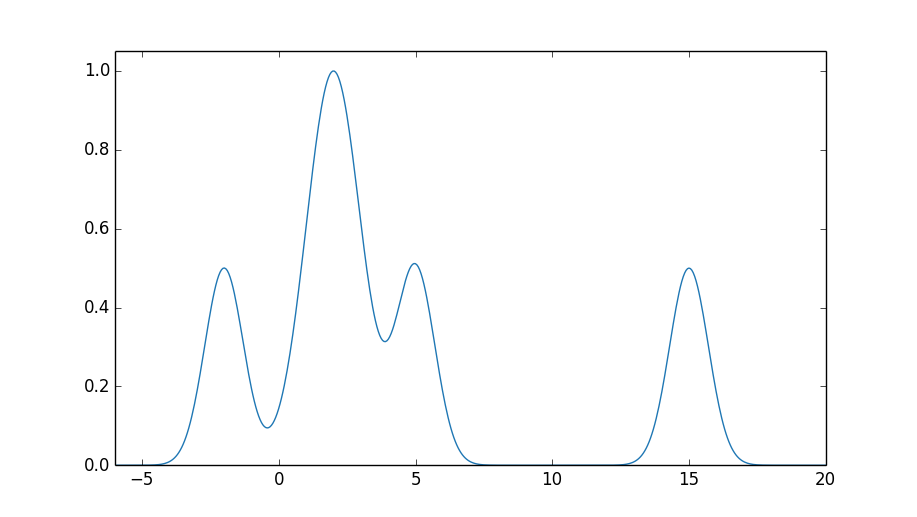
\includegraphics[width = \textwidth]{plots/function.png}
\caption{Distribution of interest}
\label{function}
\end{center}
\end{figure}

We focused on three metrics in assessing the performance:
\begin{itemize}
\item Average absolute error by number of particles. 
\item Average absolute error by wall time. 
\item Number of particles until convergence to within 2\% of the true value. 
\end{itemize}

To understand the metrics, consider Figure \ref{convergence} which shows a typical run of the two samplers where we are trying to estimate the mean of the function shown in Figure \ref{function}. The absolute value is large for both samplers within the first 10 000 iterations and before converging to within 2\% of the true value. In this particular run, the SMC sampler converged far quicker than the MCMC sampler, but each run is quite sensitive to the random seeds used. To avoid this, we average the absolute error over 50 experiments. \\

By considering the performance relative to the number particles, we overstate the performance of the SMC Sampler because it takes far longer to generate the particles (we anneal the sample from an easy distribution to the hard one). To address this computational constraint, we also compare performance relative to average wall time. Again, we average the wall time over all 50 experiments to smooth minor variances over individual runs. \\


\begin{figure}[htbp]
\begin{center}
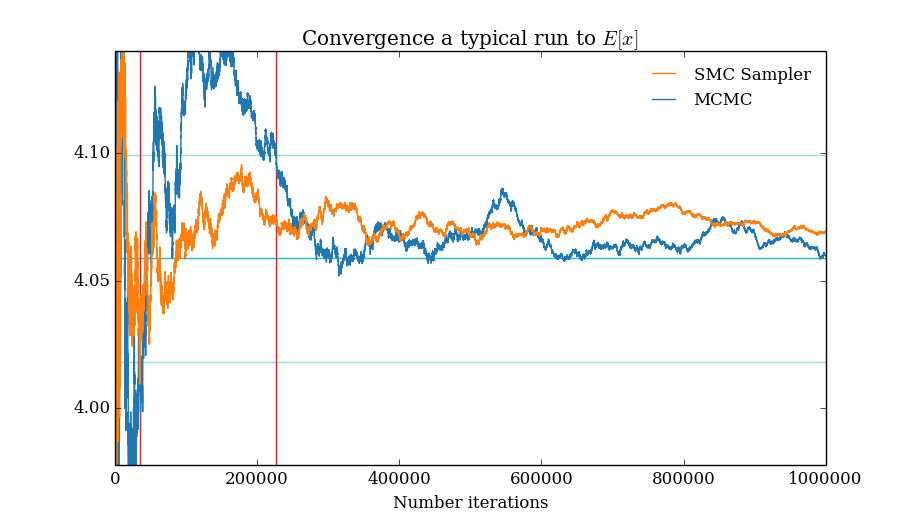
\includegraphics[width = \textwidth]{plots/Convergence.png}
\caption{Converge of a single run of MCMC and SMC. In this run SMC converged to within 2\% of the true value after 35 717 iterations and MCMC converged after 226 887 iterations (indicated by the red vertical lines)}
\label{convergence}
\end{center}
\end{figure}

Finally, by considering average performance over 50 runs, we potentially miss poor performing random draws. To understand tail performance, we consider the number of particles sampled before the chain stays within 2\% of the true value. In Figure  \ref{convergence}, for example, the MCMC estimate of the mean is within 2\% of the true value frequently within the first 1 000 iterations, but only stays within the bound for the remainder of the run after 226 887 iterations. In practice, it may be too expensive to run 50 experiments, so we would like to be confident that we have converged to the true value after a given number of iterations. To capture this we also examine the number of iterations before stabilising within 2\% of the true value for each run.

\section*{Results}
\subsection*{MAE by number of particles}
Figure \ref{ex} shows the performance of MCMC and the SMC sampler in estimating the $E[x]$ by the mean absolute error (MAE) by number of particles. It is quite apparent that the SMC sampler shows the largest improvement in absolute error over MCMC when the number of particles initiated are below 600 000. With the number of particles above 600 000, errors of both samplers appear to be converging to one another where only a negligible improvement with the SMC sampler exists.



\begin{figure}[htbp]
\begin{center}
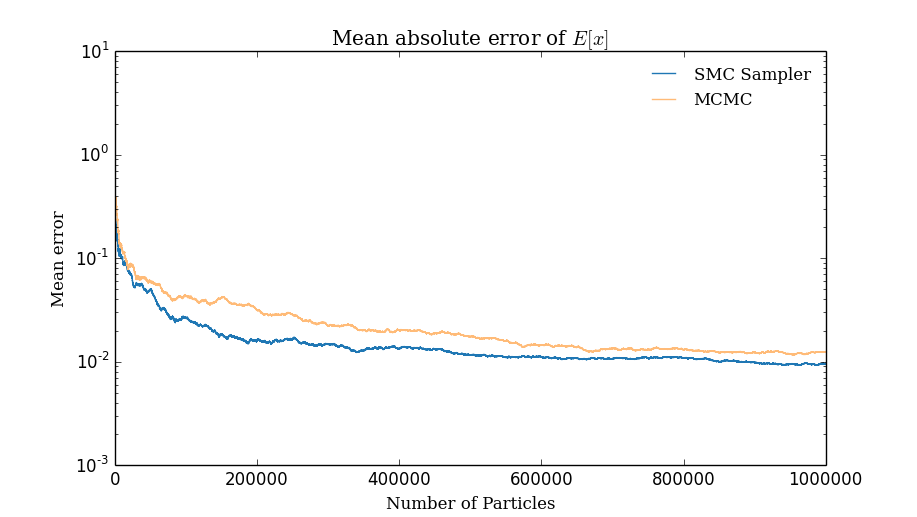
\includegraphics[width = \textwidth]{plots/E_X.png}
\caption{Performance by number of particles of the two samplers in estimating the mean.}
\label{ex}
\end{center}
\end{figure}

\begin{figure}[htbp]
\begin{center}
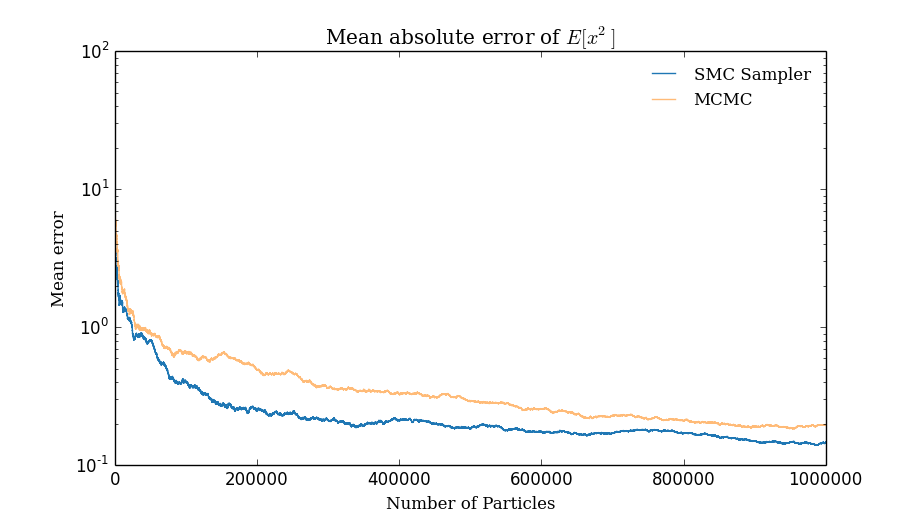
\includegraphics[width = \textwidth]{plots/E_X2.png}
\caption{default}
\label{default}
\end{center}
\end{figure}

\subsection*{MAE by wall time}
Due to the computational constraint of the SMC sampler outlined in the Convergence Benchmarks section, Figure ?? presents the average wall time over all 50 experiments.

\begin{figure}[htbp]
\begin{center}
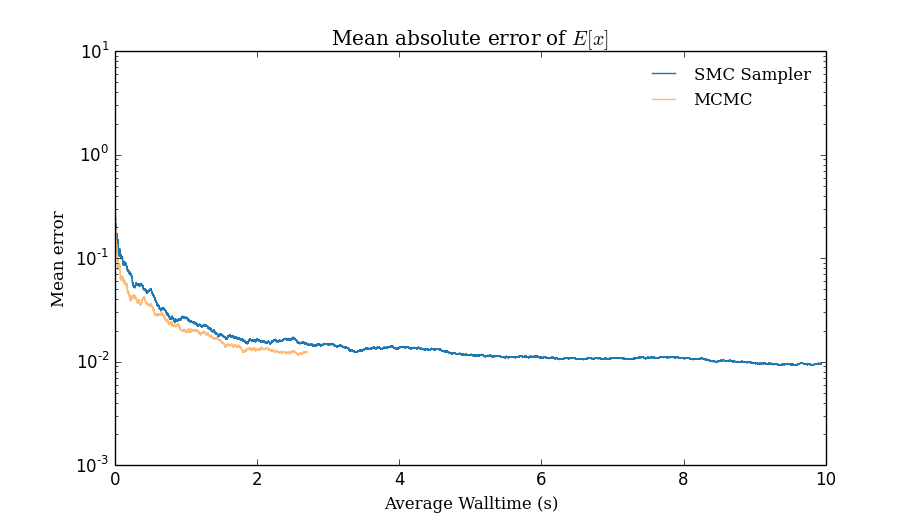
\includegraphics[width = \textwidth]{plots/E_X_walltime.png}
\caption{default}
\label{default}
\end{center}
\end{figure}

\begin{figure}[htbp]
\begin{center}
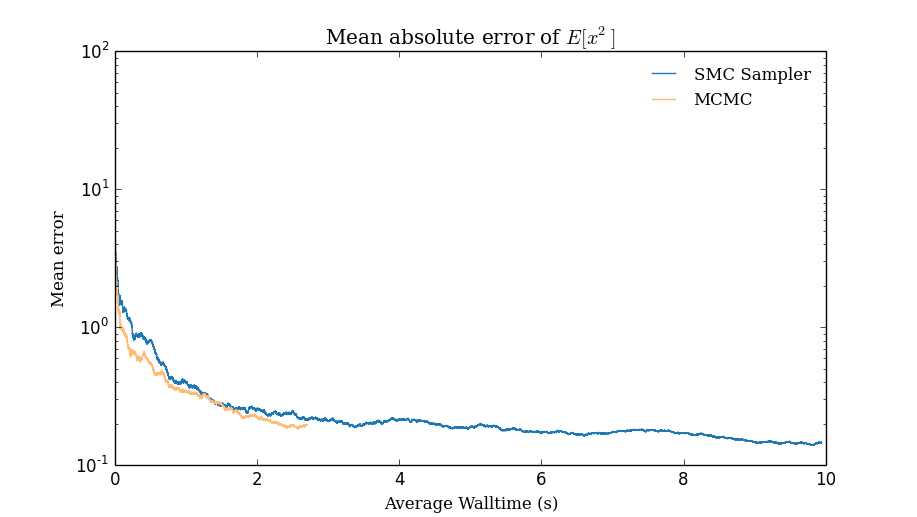
\includegraphics[width = \textwidth]{plots/E_X2_walltime.png}
\caption{default}
\label{default}
\end{center}
\end{figure}

\subsection*{Number of particles until convergence }

\begin{figure}[htbp]
\begin{center}
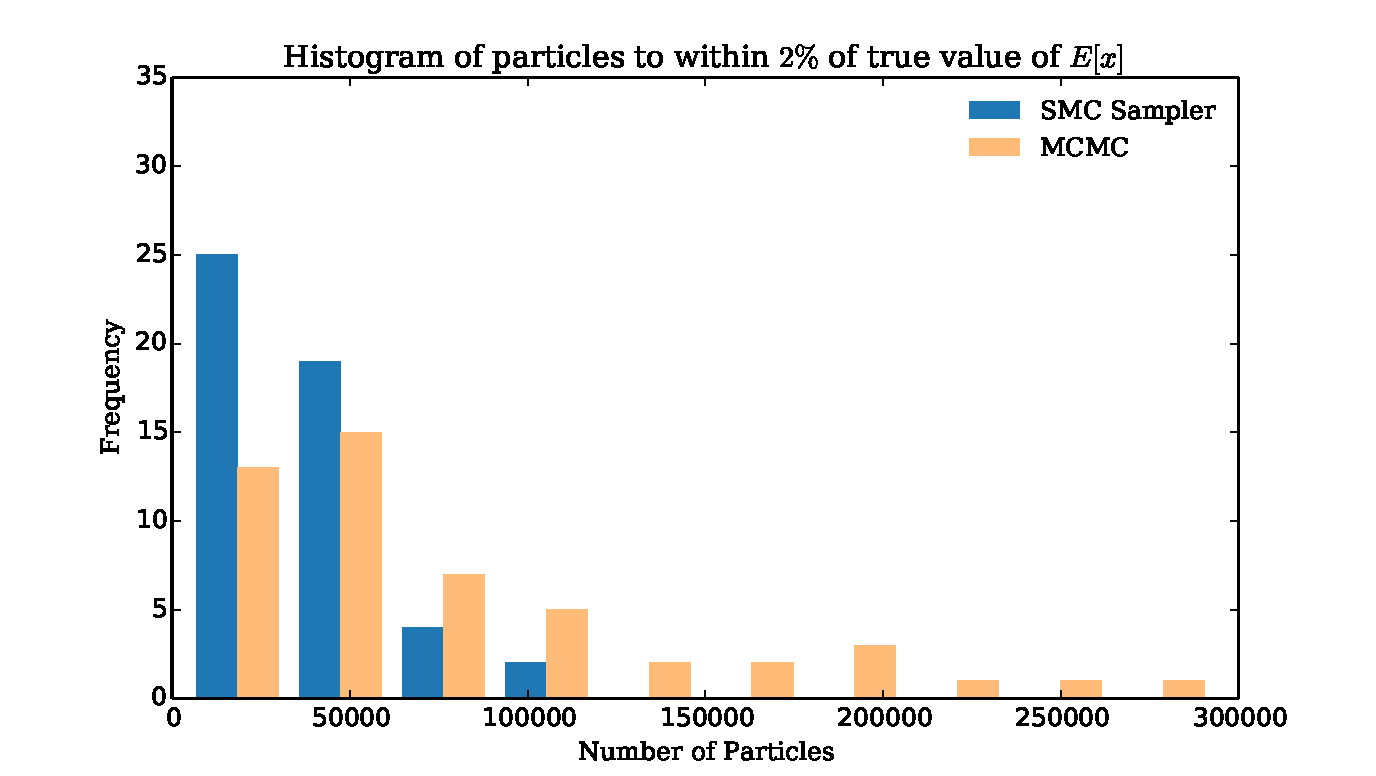
\includegraphics[width = \textwidth]{plots/iterations.pdf}
\caption{The number of iterations before the sampler converged to within $2\%$ of the true value in each of 50 experiments.}
\label{fig:itersEX}
\end{center}
\end{figure}

\begin{figure}[htbp]
\begin{center}
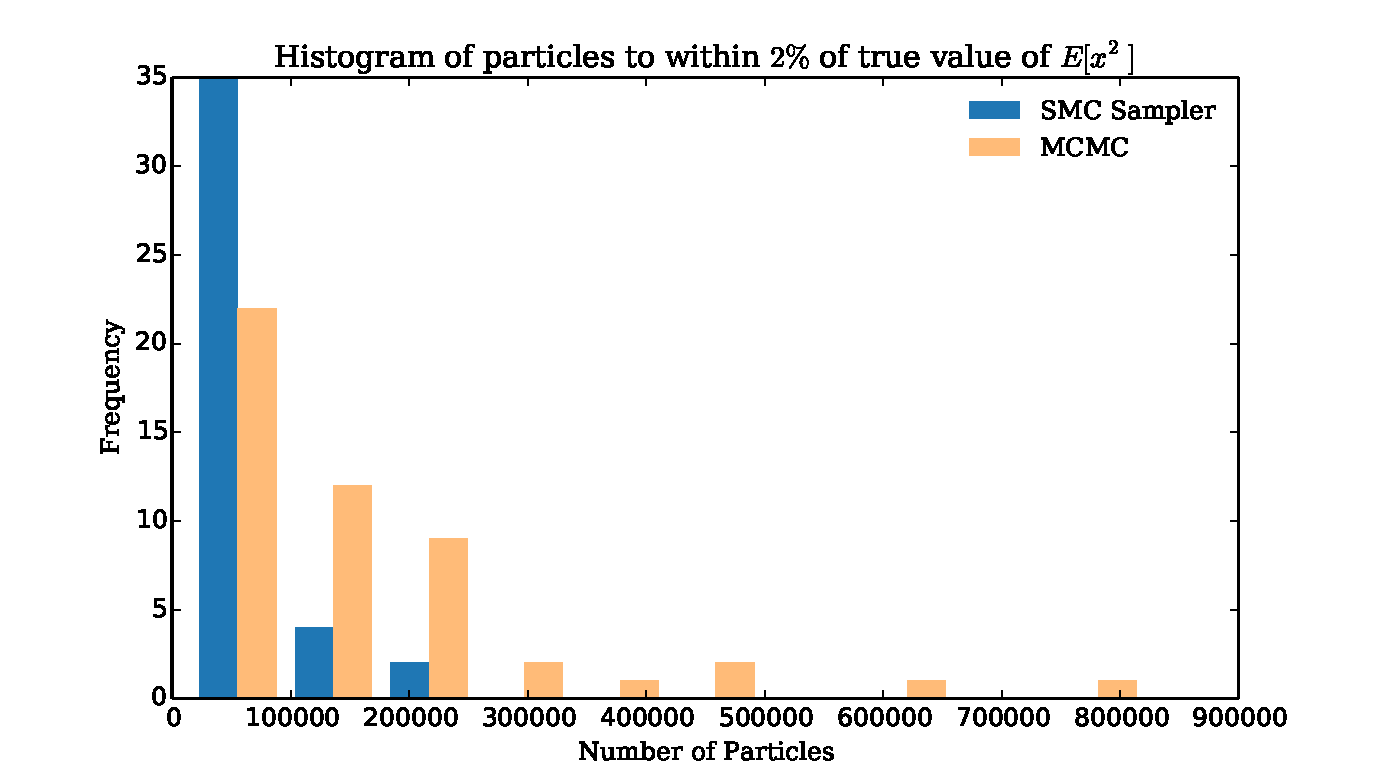
\includegraphics[width = \textwidth]{plots/iterationsEx2.pdf}
\caption{The number of iterations before the sampler converged to within $2\%$ of the true value in each of 50 experiments.}
\label{ig:itersEX2}
\end{center}
\end{figure}



\section*{Concluding Remarks}
This paper has outlined the benchmarked comparison of MCMC and SMC smplers to evaluate a series of complex artificial density functions with varying dimensions. The purpose of this comparison is to identify which sampler outperforms the other in terms of computational feasibility and convergence error. It is clear from each experiment conducted, regardless of the dimensionality, that SMC saplers converge in remarkably less iterations and a lower mean absolute error than the MCMC sampler, as denoted in Figure \ref{convergence}. \\

\subsection*{Limitations}
Despite the improved convergence results, the computational time to perform the SMC sampler is far greater than the typical MCMC approach. This may lead one to lean toward MCMC in higher dimensional space where computationally expensive experiments render the SMC sampler infeasible.

\subsection*{Further Investigation}
Due to time limitations of this paper, interesting areas relating to sampling of nonparametric Bayesian models were left unanswered. The growing interest in nonparametric Bayesian analysis has lead to increasing demands for high-performing samplers for posterior estimation, therefore providing an intriguing setting to benchmark the SMC and MCMC samplers. There is plentiful material outlining MCMC methodologies in various applied settings, but little investigation has been demonstrated through the much newer SMC smplers. Further areas of research into various applications may find SMC saplers to be highly valuable in specific scenarios where complex, multi-modal distributions pose a difficulty for the conventional MCMC sampler.


\bibliographystyle{model1-num-names}
\bibliography{sample.bib}

\end{document}